\section{Accelerator Model}

The block diagram of \figurename~\ref{fig:acctile} illustrates the ESP
accelerator socket and shows the three main set of signals at the interface of
an ESP accelerator: read and write port for data transfers through DMA requests,
configuration port and interrupt line.

\begin{figure*}[h]
  \vspace{0.2in}
  \centering
  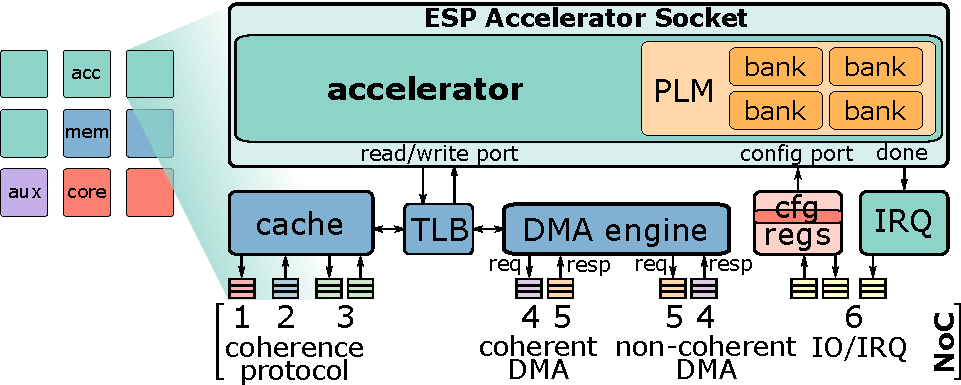
\includegraphics[width=0.65\textwidth]{../fig/acctile.pdf}
  \label{fig:acctile}
  \caption{Block diagram of ESP accelerator tiles}
\end{figure*}

A typical ESP accelerator is composed of three control blocks
({\it configuration, load, store}), one or more computation blocks and a
customized private local memory (PLM).

Once configuration registers are valid, the configuration block activates the
other components. The {\it load} module initiates the first DMA transaction to
fetch the input data, or a portion of it, from the system memory hierarchy into
the PLM. Next, the computation blocks process the available input and produce
the corresponding output. Finally, the {\it store} block writes back the output
to the system memory hierarchy with a DMA request. A single accelerator
invocation from software typically results into multiple iterations of {\it
  load}, {\it compute} and {\it store} phases, therefore we
recommend implementing a portion of the PLM as a set of ping-pong buffers to
enable pipelining.
Depending on the particular task and accelerator implementation, this strategy
may significantly improves the overall accelerator throughput by masking most of
the time for data transfers with the overlapping computation steps.

The above accelerator model corresponds to what ESP automation provides
through any of the available high-level synthesis flows. RTL designers are not
required to follow these directions, as long as they comply with the
signal-level protocol at the interface with the ESP socket.


\subsection{Accelerator Configuration}

The configuration block regulates the accelerator execution and implements the
interface with software by sampling the value of common and user-defined
configuration registers located in the ESP socket.

\begin{table}[h!]
\centering
\small
\caption{Description of the ESP accelerator configuration port.}\label{tab:acc_cfg}
\begin{tabular}{|p{2.25in} p{0.75in}| p{3.25in} |}
\hline
  \textbf{Signal}         & \textbf{Driver} & \textbf{Description} \\
\hline
  \verb clk  & socket & accelerator clock. \\
\hline
  \verb rst & socket & accelerator reset {\bf active low}. The socket activates
                       this reset signal when software clears the interrupt
                       request to ensure that the accelerator is ready for a new
                       invocation and internal state is clean. If the
                       accelerator is expected to retain its state across
                       different invocations, a user-defined configuration
                       register can be used to implement a software-controlled
                       reset signal. \\
\hline
\verb conf_done & socket & Configuration registers are valid and computation can
                           start. This signal is active high and asserted for
                           one \texttt{clk} cycle to trigger the accelerator
                           execution. \\
\hline
\verb conf_info_<register_name> & socket & User-defined configuration input. The
                                           corresponding memory-mapped
                                           configuration registers are
                                           automatically generated in the ESP
                                           socket when creating the SoC
                                           instance. There can be up to 14
                                           user-defined registers that must be
                                           listed in the accelerator definition
                                           XML file (see Section~\ref{sec:xml}
                                           For each register the accelerator
                                           must expose one \texttt{conf\_info\_}
                                           input. Bitwidth must be between 1 and
                                           32 bits. These inputs should be
                                           considered valid when the
                                           \texttt{conf\_done} input is active
                                           high. \\
\hline
  \verb acc_done  & accelerator & Single-cycle pulse active high. This flag
                                  indicates that the accelerator has completed
                                  its task. The pulse should occur only after
                                  the last DMA write transaction has completed
                                  and all output data have been transferred from
                                  the PLM to the memory hierarchy. Asserting
                                  \texttt{acc\_done} will trigger an interrupt
                                  request to the interrupt controller located
                                  in the ESP auxiliary tile. The software
                                  interrupt handler is responsible for clearing
                                  the interrupt, thus resetting the state of the
                                  socket and activating the \texttt{rst} input
                                  of the accelerator. \\
\hline
  \verb debug  & accelerator & 32-bit debug output. The accelerator designer can
                               use this output to encode error codes. The state
                               of this output can be accessed through the common
                               memory-mapped registers present in the socket. \\
\hline
\end{tabular}
\end{table}

\subsection{Private Local Memory}
The PLM can be generated with the ESP \texttt{Memgen} utility, which combines
SRAM primitives available as part of the target technology libraries.
Alternatively, the accelerator designer can manually implement the PLM in RTL.

The PLM is not memory mapped, hence it is not exposed to software. Furthermore,
the PLM is not part of the SoC cache hierarchy as it is solely intended as a
customized working buffer for the accelerator data path.
%
As a result the PLM has no external interface exposed to the ESP accelerator
socket and RTL designers are not required to comply with any hierarchy
convention or signal-level protocol to implement the PLM, unless using the ESP
\texttt{Memgen} utility (refer to the \texttt{ESP Memory Generator}
documentation for further information).
Accelerators that operate on small batches of data and don't have particular
buffering requirements can also be implemented without a PLM.

